\chapter{One-dimensional computational RICS}
\lettrine[lines=2, lhang=0.33, loversize=0.25]{A}{ccording to our
analysis,} profound barriers to diffusion exist in
cardiomyocytes. To test whether it is possible to localize such
diffusion obstacles in \ac{RICS} measurements we again turned to mathematical
modelling. 

\label{ch:1d_comp_res}
\section{Motivation \& model setup}
So far in this dissertation, \ac{RICS} analysis has been performed and
\acp{DC} estimated from the entire region acquired in either experiment
or computational model. Here, a different approach is used.
One-dimensional \ac{RICS} simulations are performed as previously (see
\ref{ch:comp_res} and \PaperIII). Two barrier-to-barrier
distances (5 and 1 $\mu$m) and several barrier permeabilities (p) ranging from 0 to
75\% are used as model parameters. Molecules diffuse in the \acl{IBS}
with a given \ac{DC} ($D_{IBS}$) in one dimension. When
coming in contact with a barrier they can either pass through the
barrier or bounce back. The probability of doing either is determined by
the permeability of the barrier. The computational model produces linescan images of a
20 $\mu$m region. In subsequent processing the region is divided into
smaller subregions and \ac{RICS} analysis is performed on each of these
independently and apparent \acp{DC} found ($D_{app}$). For comparison, analysis on the whole 20 $\mu$m region is
performed also, similarly to the analysis in \ref{ch:comp_res}.

\begin{figure}[t!]
  \centering
    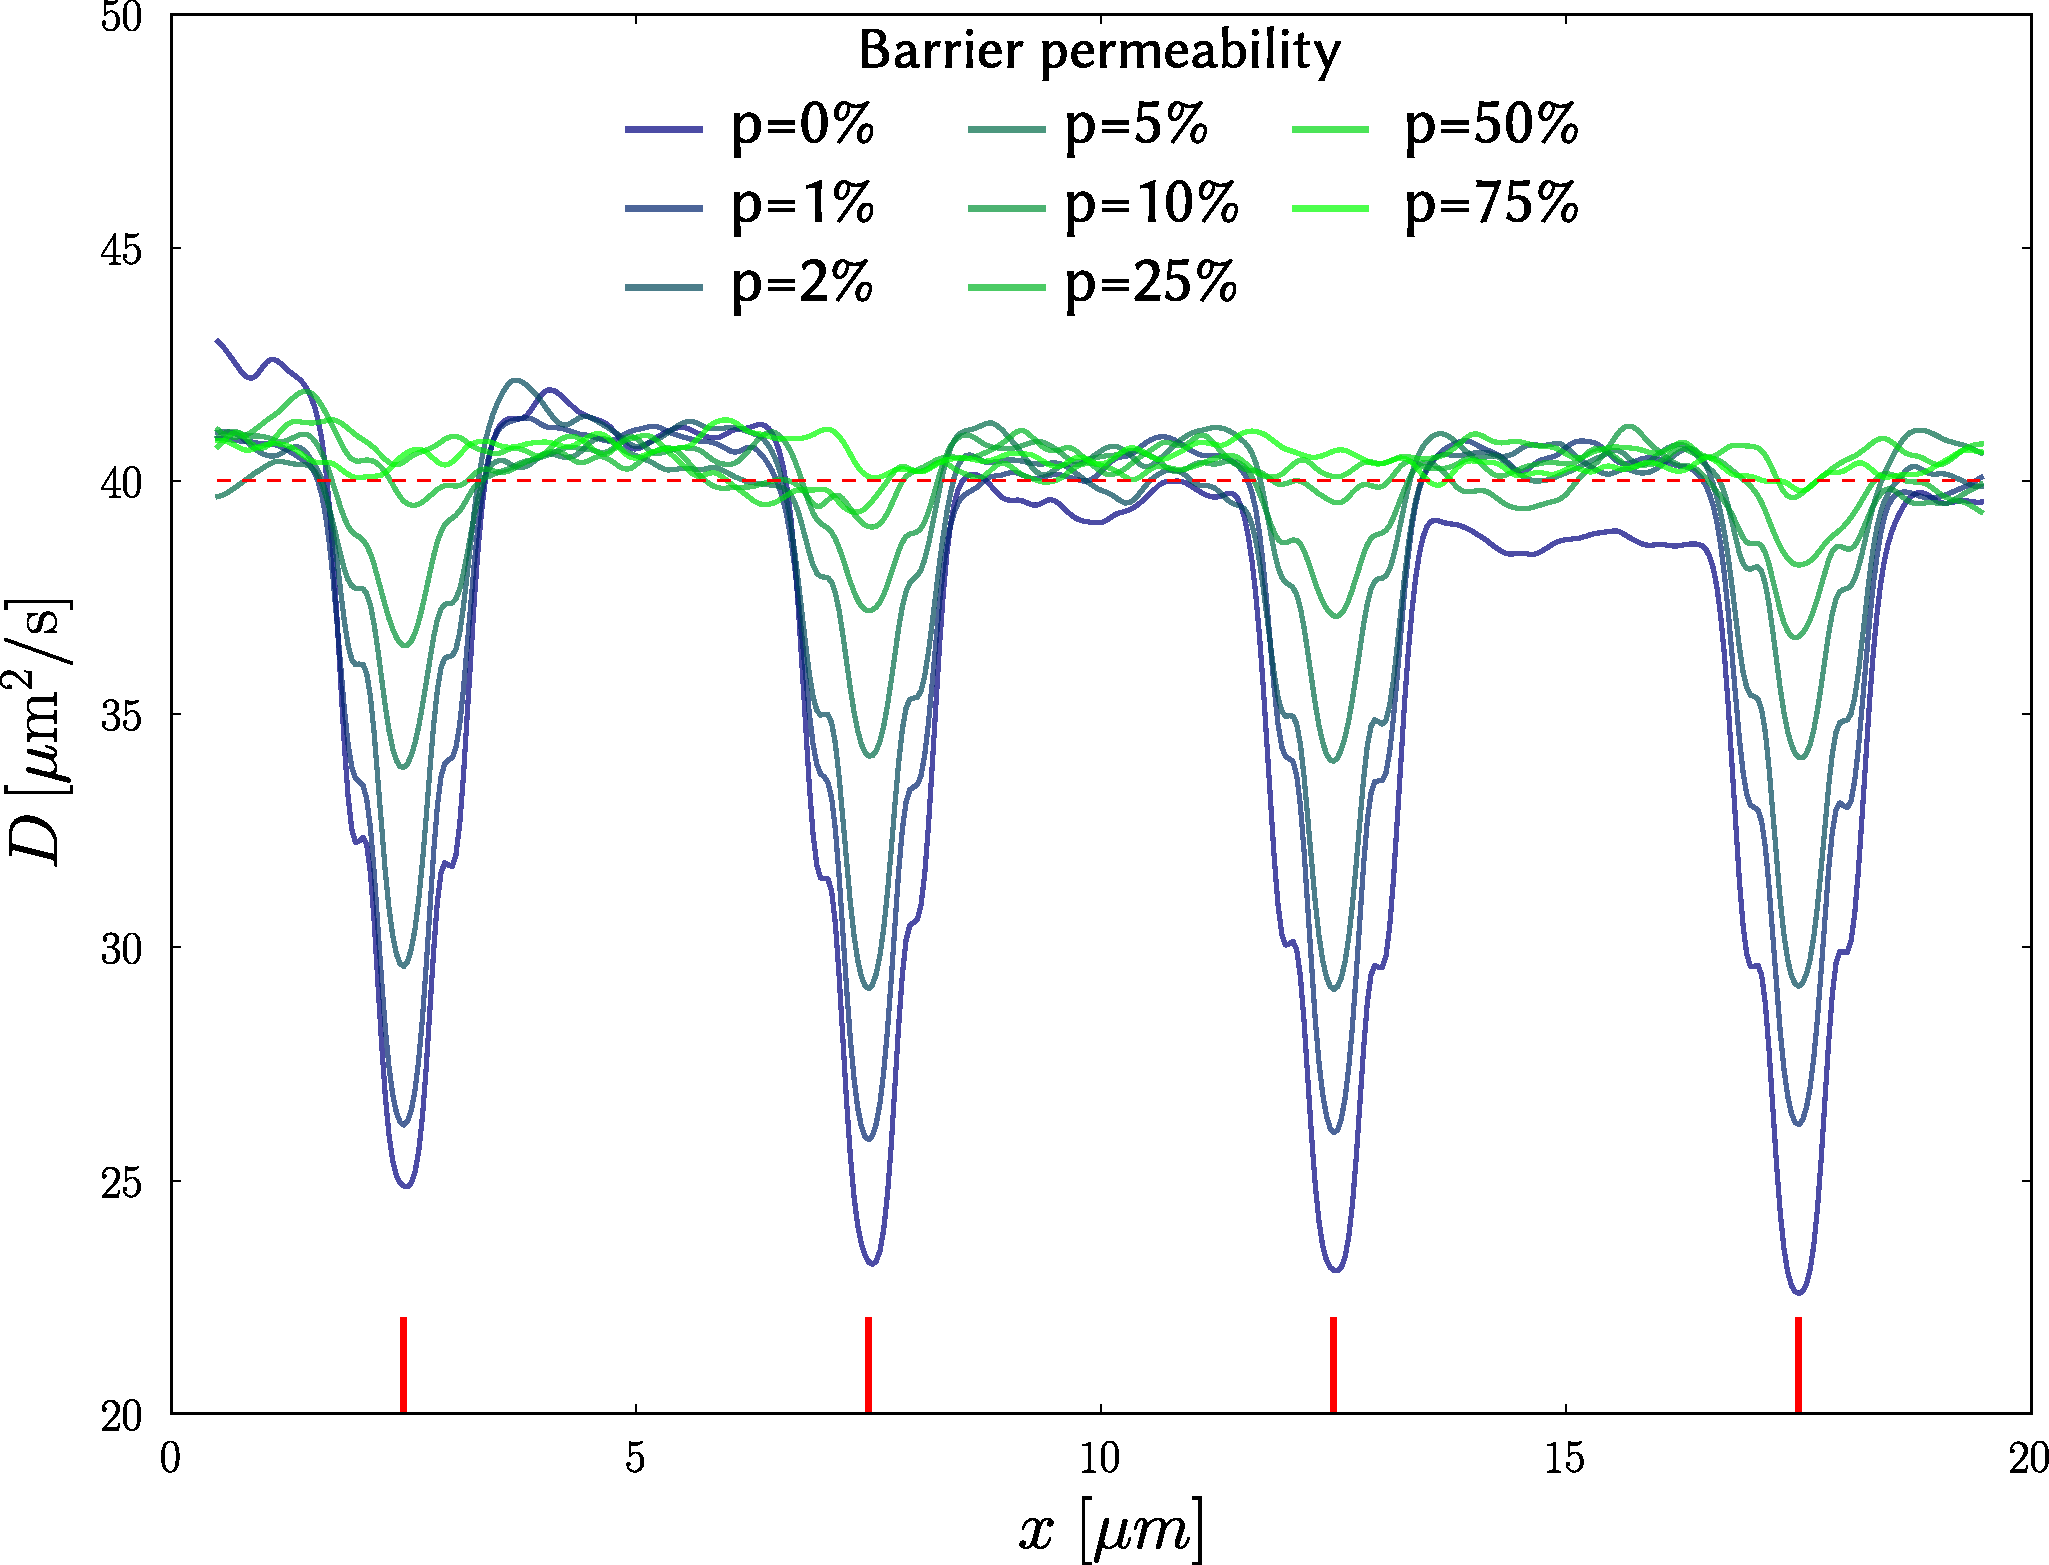
\includegraphics[width=9cm]{figures/range_5.pdf}
    \caption[Regional \acsp{DC} for barriers 5 $\mu$m apart]{\acsp{DC} obtained from regional \ac{RICS} analysis
    of linescan data obtained from a computational model. Barriers
    (indicated by short vertical lines) are places 5 $\mu$m apart and
    their permeability(p) is varied between model runs. \acsp{DC} obtained
    for varying permeability values are shown with different lines. The
    value shown at any $x$ location is the \ac{DC} obtained from
    \ac{RICS} analysis on the 1 $\mu$m segment centered at that
    location.}
    \label{fig:1drange}
 % \label{fig:rics_theory1}
%The autocorrelation at shift vector $\Delta \mathbf{h}=(\xi,\psi)$ for an image with
%fluorescence values $F(\mathbf{p})$ at location $\mathbf{p} = (x,y)$ is given by:
%{\small
\end{figure}
\section{Barrier effects on regional diffusion coefficients}
From performing the regional analysis described above, a sequence of
\acp{DC} can be obtained. An example of simulation and regional analysis
results is presented on \F{~\ref{fig:1drange}}. Here, the \ac{DC} in the \ac{IBS} is set to
$D_{IBS}=$40$\mu$m$^2$/s and within the 20 $\mu$m space there are 4
barriers restricting diffusion, placed at 5 $\mu$m from each other. The
permeabilities of these barriers are varied in order to study the effect
of permeability on the estimated apparent \acp{DC} obtained from
\ac{RICS} analysis. Results obtained for a range of barrier permeability
values are represented by different curves in \F{~\ref{fig:1drange}}. It
is visible that the apparent \ac{DC} reduces almost twofold in regions
with a barrier in the center.

The relative decrease in \ac{DC} ($\sfrac{\Delta
D}{D_{IBS}=\sfrac{(D_{IBS}-D_{APP})}{D_{IBS}}}$), calculated for the region around a single barrier
is averaged for equivalent neighbourhoods around each barrier and the curves shown in
\F{~\ref{fig:walls_xi}A} are obtained.
The solid horizontal line indicates the position of the barrier, dashed lines show the 5 $\mu$m
region centered at the barrier. It can be seen from the plot that even
in cases when the region used for \ac{RICS} estimation does not include
the barrier (\ie, any point outside of the dashed lines), the barrier
still affects the \ac{DC}. 

A similar analysis for a model with barriers
separated by 1 $\mu$m is shown on \F{~\ref{fig:walls_xi}B}. In this case
the region used for \ac{RICS} analysis is limited to 1 $\mu$m but is plotted on the same scale
as \F{~\ref{fig:walls_xi}A} to make comparison easier. Compared to the
5 $\mu$m barrier distances on \F{~\ref{fig:walls_xi}A}, the presence of 
more closely placed barriers causes a decrease in the apparent \ac{DC}
further away from the barrier.
%Also, an interesting effect is visible as barrier permeabilities approach 0. In such a case
%diffusing particles are effectively trapped in between the barriers,
%resulting in the estimated \ac{DC} being reduced less than when the
%barrier is only slightly less permeable (i.e., comparing 0\%
%permeability to 0.1\%).  

\begin{figure}%[h!]
  \centering
    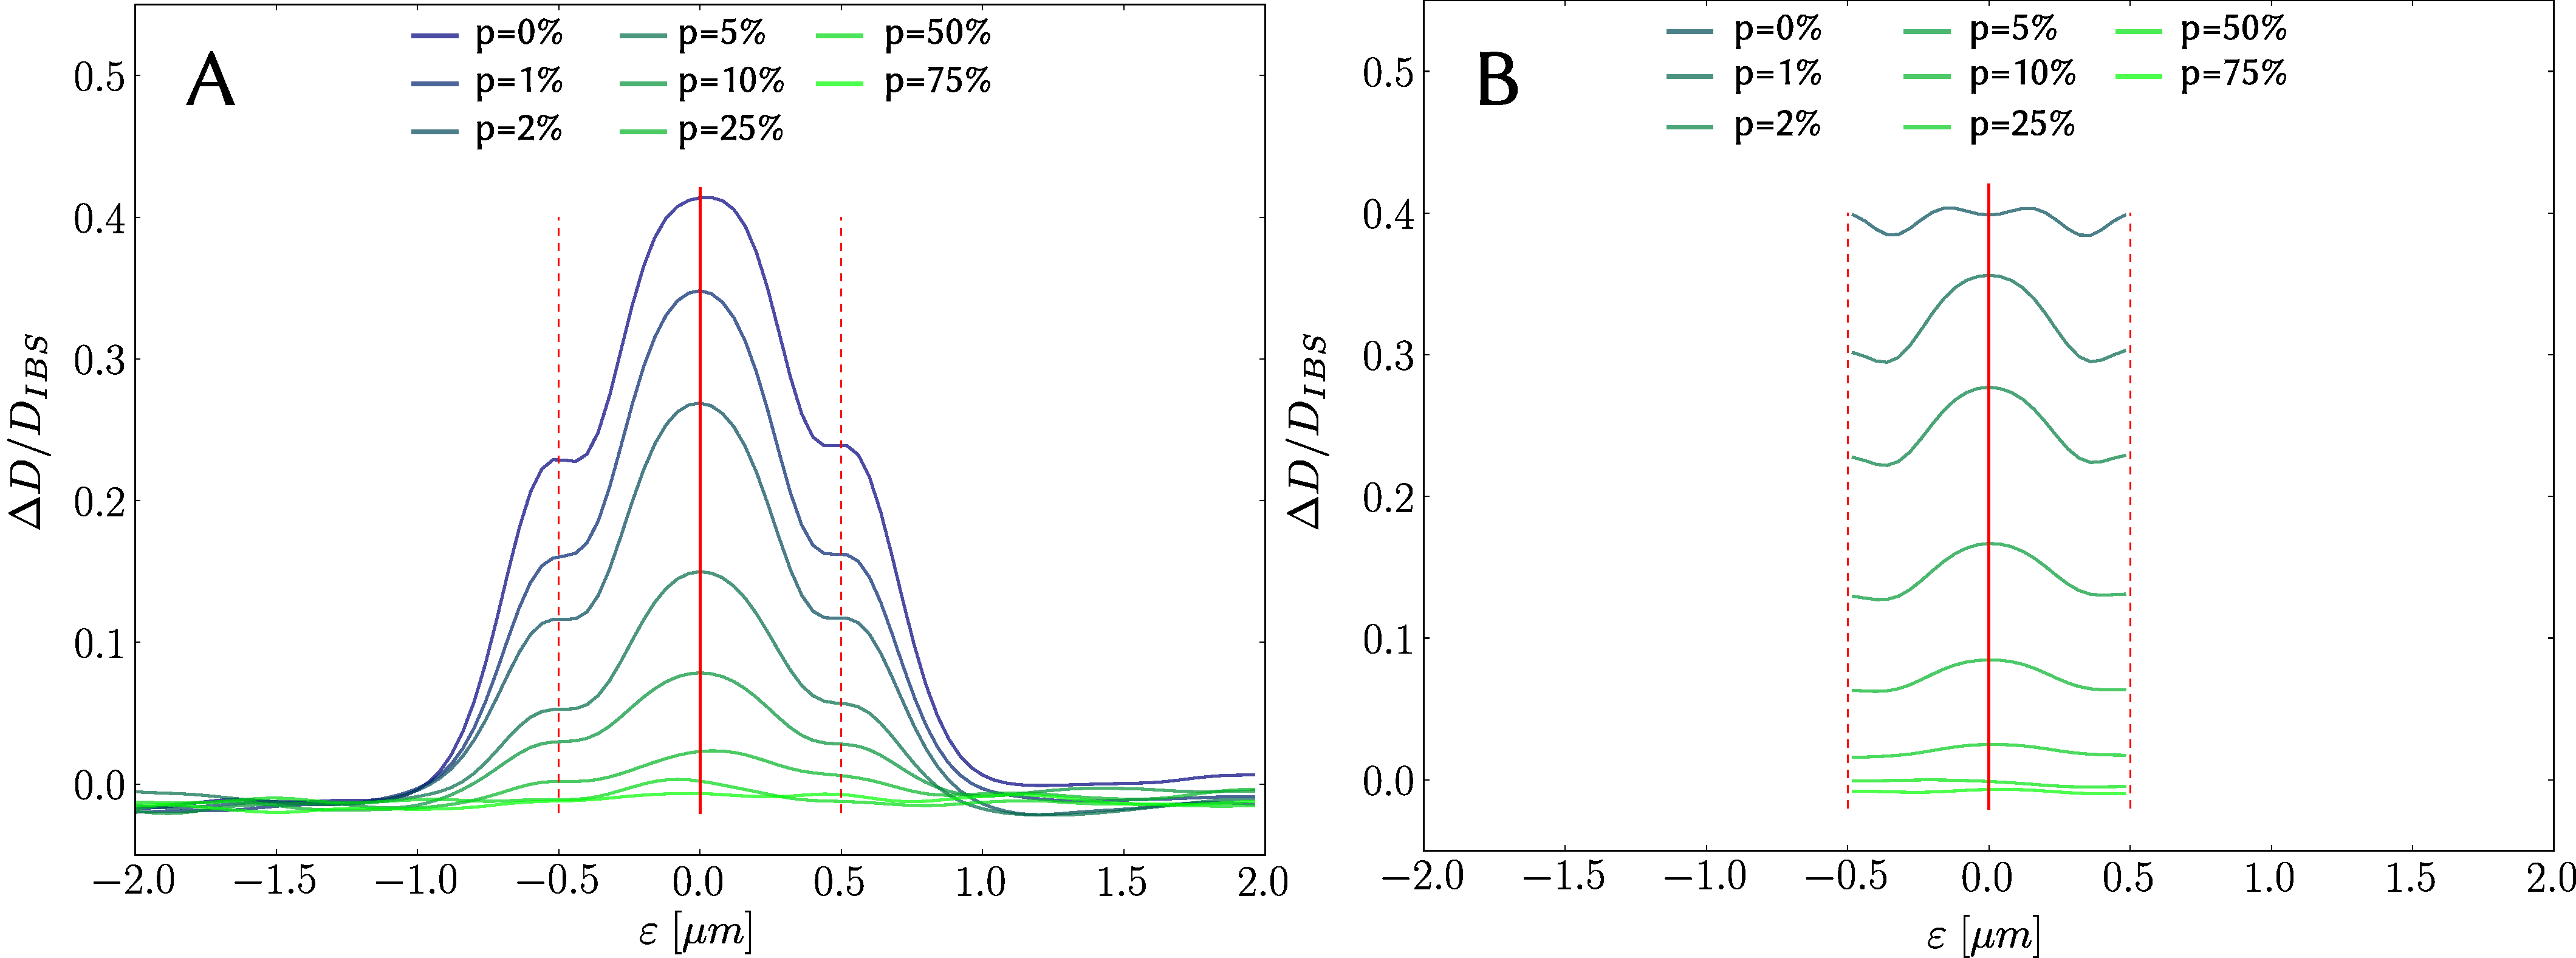
\includegraphics[width=12cm]{figures/walls_xi.pdf}
    \caption[Average relative decrease in \acs{DC} for barriers 5 and 1 $\mu$m apart]
    {(A) Average relative decrease in \acs{DC} at various barrier
    permeabilities in the neighbourhood around a barrier for barriers
    placed 1 $\mu$m apart.  $\varepsilon$
    indicates the distance of the center of the region used for \ac{DC} estimation
    from the barrier. (B) Same as A except for barriers place 1 $\mu$m
    apart.}
    \label{fig:walls_xi}
 % \label{fig:rics_theory1}
%The autocorrelation at shift vector $\Delta \mathbf{h}=(\xi,\psi)$ for an image with
%fluorescence values $F(\mathbf{p})$ at location $\mathbf{p} = (x,y)$ is given by:
%{\small
\end{figure}
%\begin{figure}%[h!]
%  \centering
%    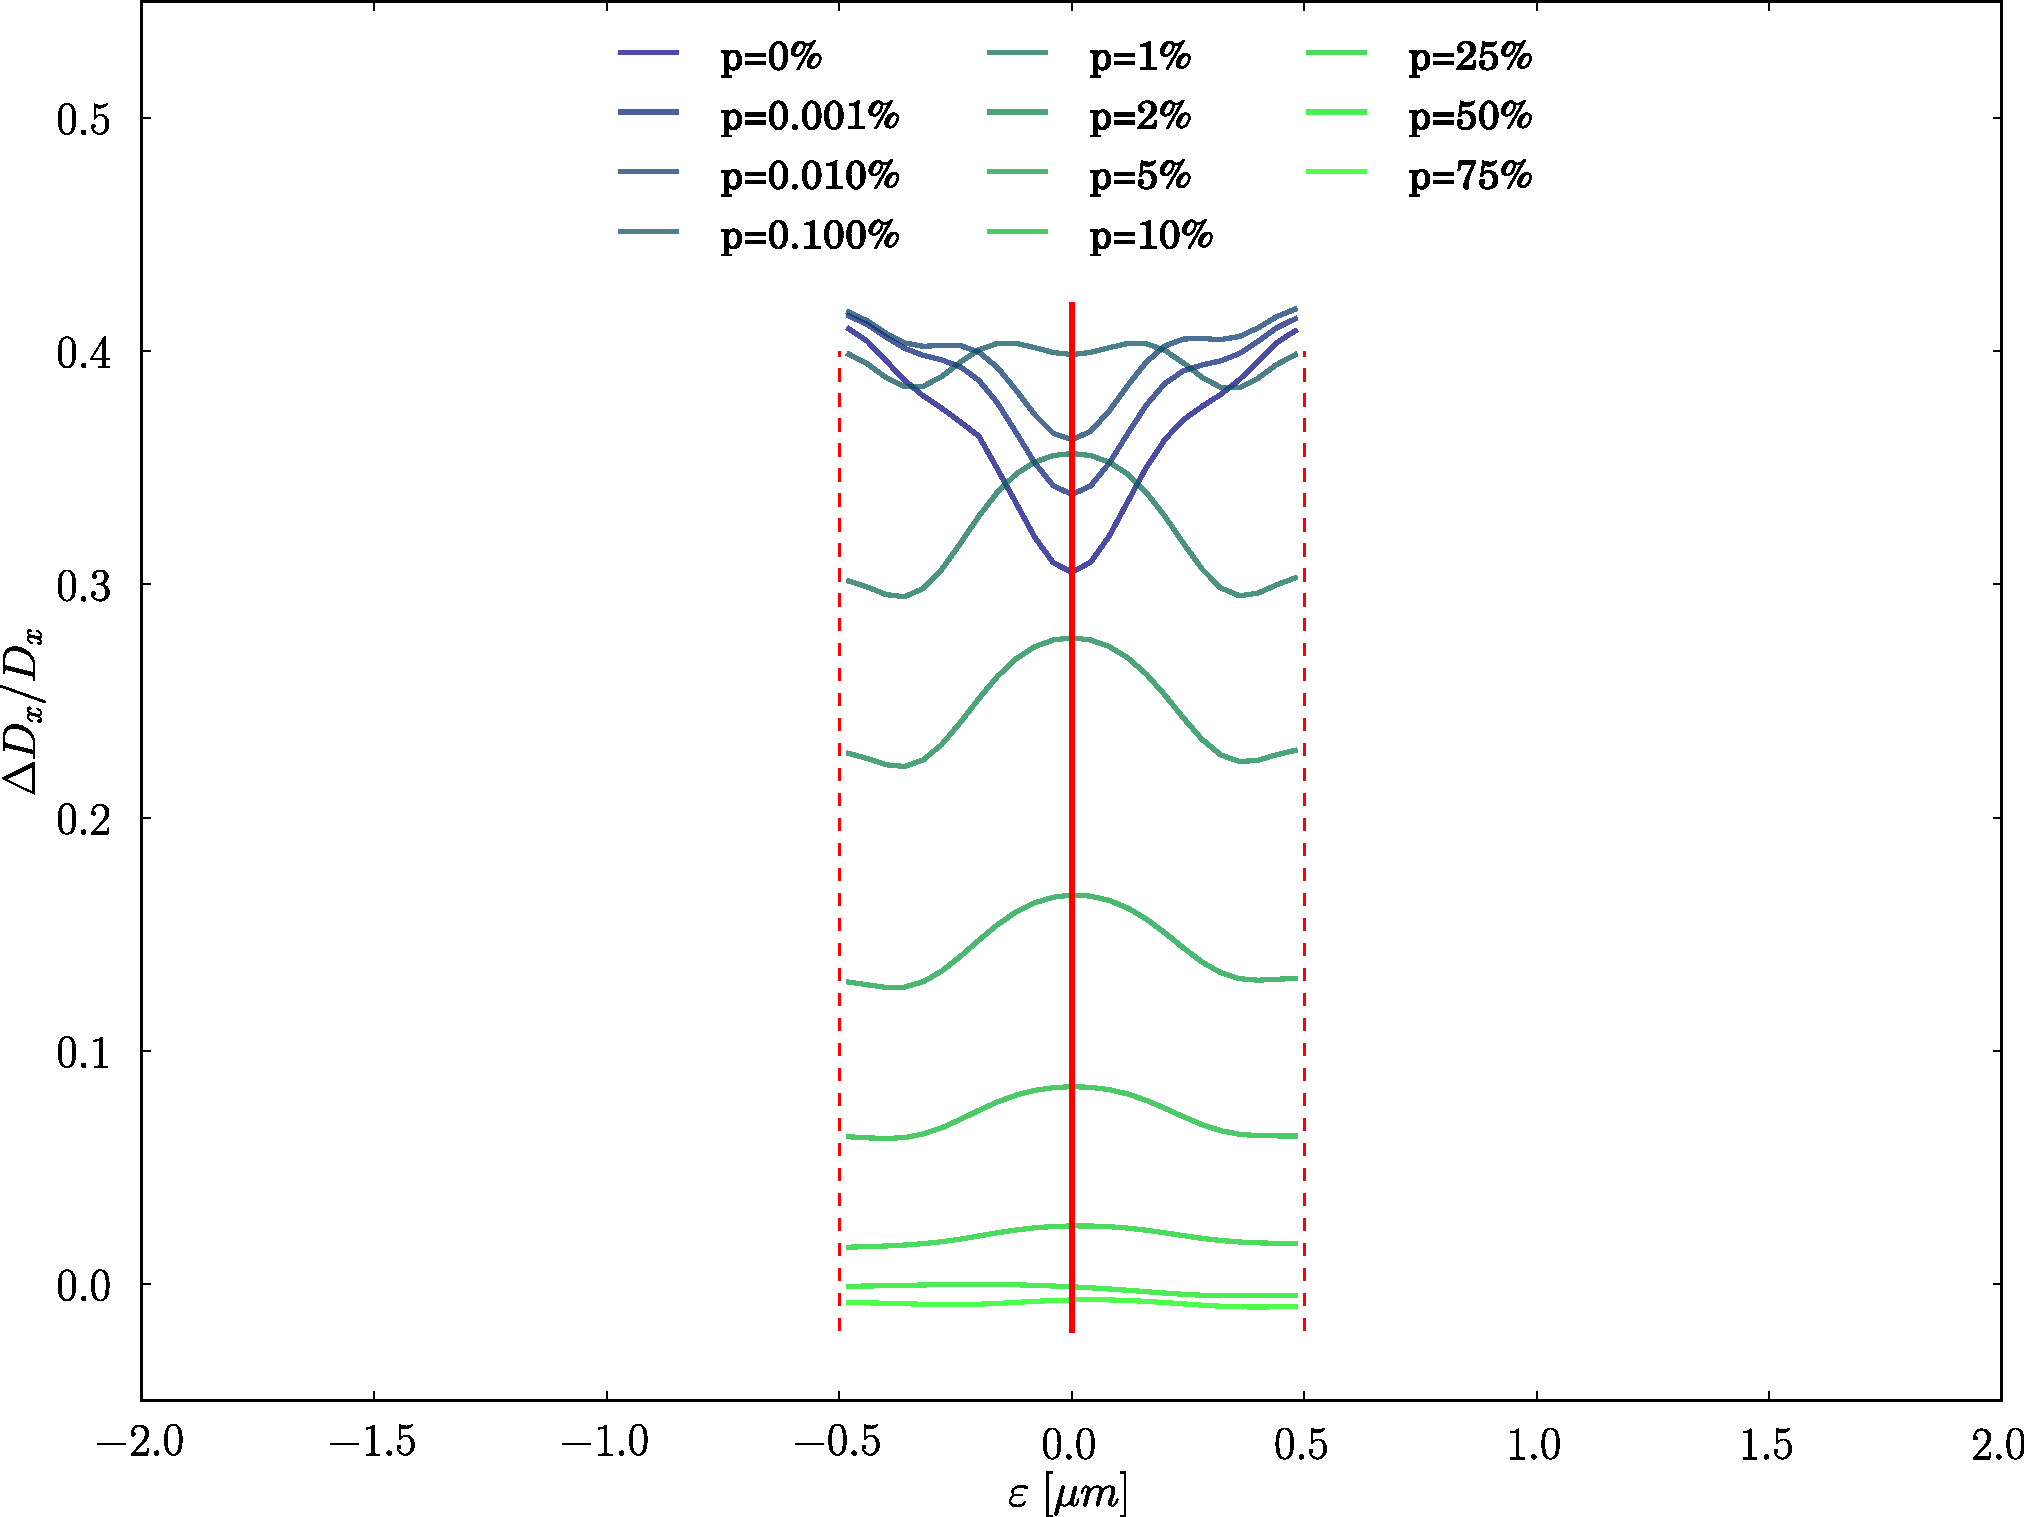
\includegraphics[width=10cm]{figures/wall_1_xi.pdf}
%    \caption[Average relative decrease in \acs{DC} for barriers 1 $\mu$m
%    apart]{Average relative decrease in \acs{DC} at various barrier permeabilities in the neighbourhood around a barrier for barriers placed 1 $\mu$m apart}
%
%    \label{fig:wall1xi}
% % \label{fig:rics_theory1}
%%The autocorrelation at shift vector $\Delta \mathbf{h}=(\xi,\psi)$ for an image with
%%fluorescence values $F(\mathbf{p})$ at location $\mathbf{p} = (x,y)$ is given by:
%%{\small
%\end{figure}
When the maximum relative decrease of \ac{DC} relative to the \ac{DC} in
\ac{IBS} is calculated as a function of permeability, the
effect of the region size used for \ac{DC} estimation in \ac{RICS}
becomes visible. On \F{\ref{fig:max_5}} curves showing the maximum relative
decrease for 3 different region sizes are plotted. From here it can be
seen that as the region size increases the effect barriers have on the
apparent \ac{DC} is lessened. When the whole image is analysed as a
single 20 $\mu$m region, the decrease in \ac{DC} is reduced compared to
all regional cases. Therefore, localized diffusion restrictions,
represented here by barriers, result in more pronounced
decreases in \acp{DC} when estimated on a smaller scale. On the large scale,
however, this effect is lessened and appears as a uniform reduction in
the apparent \ac{DC}.

\begin{figure}%[h!]
  \centering
    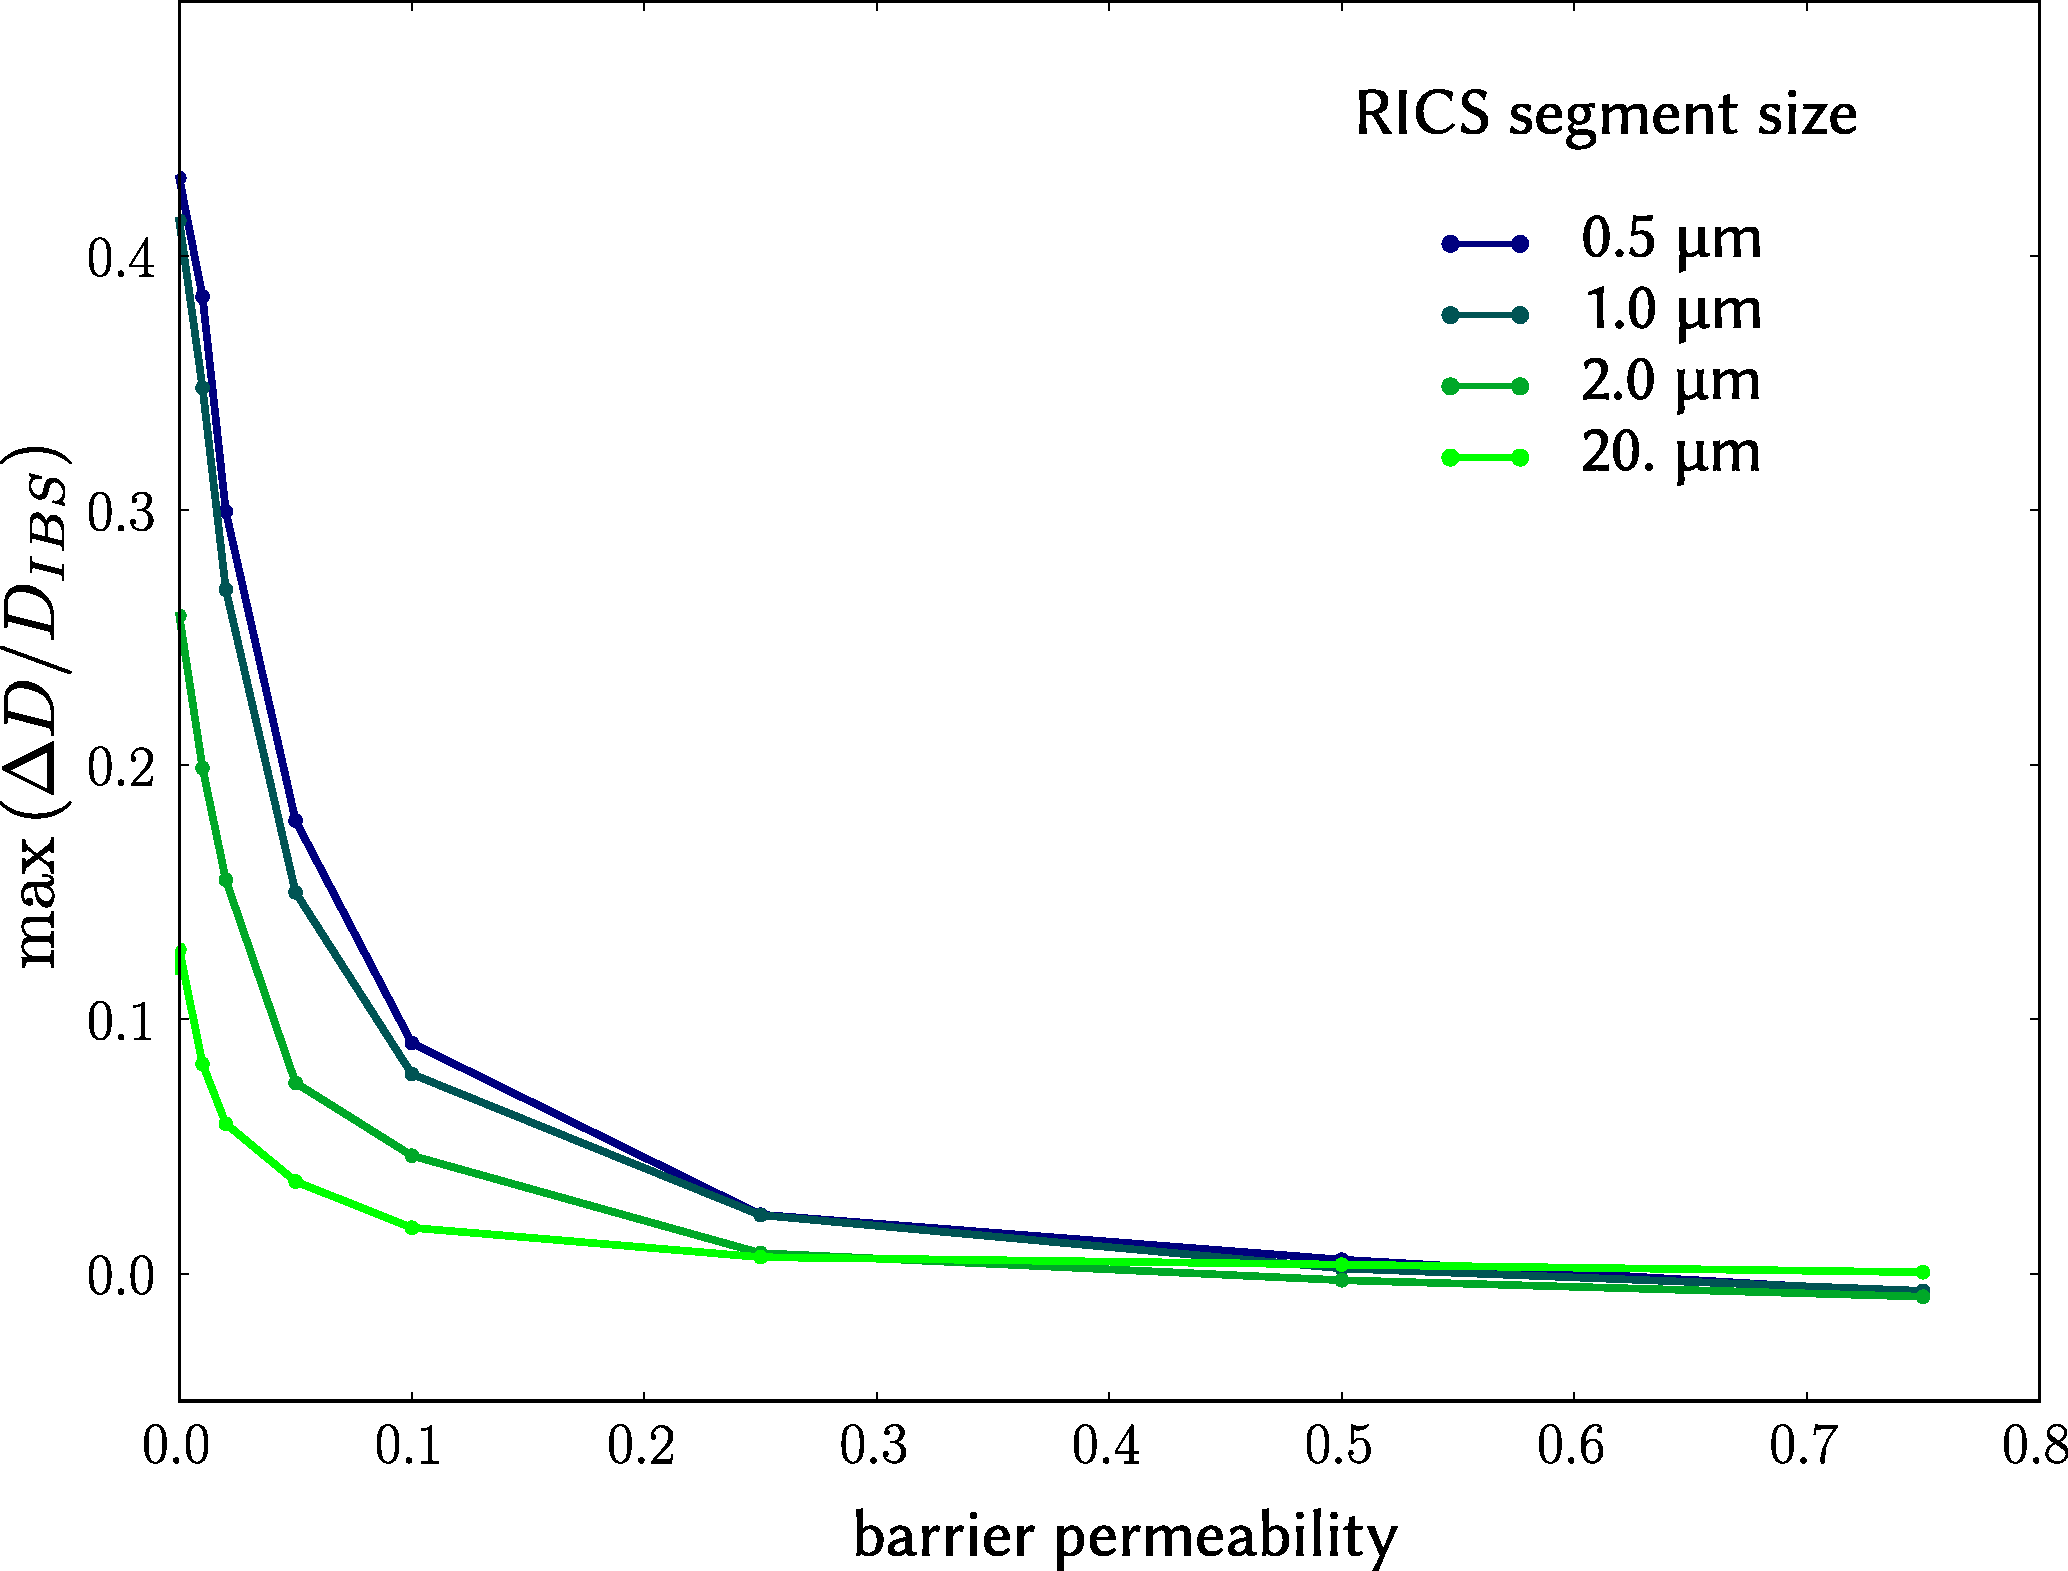
\includegraphics[width=6cm]{figures/max_5b.pdf}
    \caption[Maximum relative decrease in \acs{DC}]{Maximum relative
    decrease in \acs{DC} as a function of barrier permeability. Different
    curves indicate analysis region lengths of 2,1 and 0.5 $\mu$ m. The
    20 $\mu$m region signifies analysis performed on the entire image.}
    \label{fig:max_5}
 % \label{fig:rics_theory1}
%The autocorrelation at shift vector $\Delta \mathbf{h}=(\xi,\psi)$ for an image with
%fluorescence values $F(\mathbf{p})$ at location $\mathbf{p} = (x,y)$ is given by:
%{\small
\end{figure}
\section{Conclusions}

Applying \ac{RICS} to 1D diffusion reveals that barriers affect
estimation of \acp{DC} even if the area from which image data used
for \ac{DC} estimation was acquired does not contain a single barrier, 
but is nearby a region where a barrier is present. The distance at which this effect is observable depends on the permeability of the barrier, the \ac{DC} of the dye in the inter barrier space and the size of the segment used for apparent \ac{DC} estimation. 
